% https://tex.stackexchange.com/q/761912/322482
% https://tex.stackexchange.com/a/553445/322482
% https://tex.stackexchange.com/a/37926/322482
\documentclass[border=5pt]{standalone}
\usepackage{tkz-euclide}
\usepackage{fourier}
\usetikzlibrary{calc,arrows.meta,decorations.pathreplacing}

\makeatletter
\tikzset{
  invertdim/.style args={#1,#2,#3,#4}{%
    postaction={
      decoration={
        show path construction,
        lineto code={
          \coordinate (tkzInvertDimStart) at ($ (\tikzinputsegmentfirst)!#2!90:(\tikzinputsegmentlast) $);
          \coordinate (tkzInvertDimEnd) at ($ (\tikzinputsegmentlast)!#2!-90:(\tikzinputsegmentfirst) $);
          \coordinate (tkzInvertDimLeftOuter) at ($ (tkzInvertDimStart)!-#4!(tkzInvertDimEnd) $);
          \coordinate (tkzInvertDimRightOuter) at ($ (tkzInvertDimEnd)!-#4!(tkzInvertDimStart) $);
          \draw[invertdim fence style/.try]
            (\tikzinputsegmentfirst) -- ($ (\tikzinputsegmentfirst)!1.25*(#2)!90:(\tikzinputsegmentlast) $)
            (\tikzinputsegmentlast) -- ($ (\tikzinputsegmentlast)!1.25*(#2)!-90:(\tikzinputsegmentfirst) $);
          \path
            ($ (tkzInvertDimStart)!0.5!(tkzInvertDimEnd) $)
            node[inner sep=0pt, font=\footnotesize, fill=\tkz@fillcolor, #3] (tkzInvertDimLabel) {#1};
          \draw[invertdim style/.try] (tkzInvertDimLeftOuter) -- (tkzInvertDimStart);
          \draw[invertdim style/.try] (tkzInvertDimRightOuter) -- (tkzInvertDimEnd);
        }
      },
      decorate,
    }
  },
  invertdim/.default={,0pt,,6pt},
  invertdim style/.style={thick,-latex},
  invertdim fence style/.style={thick},
}
\makeatother

\begin{document}
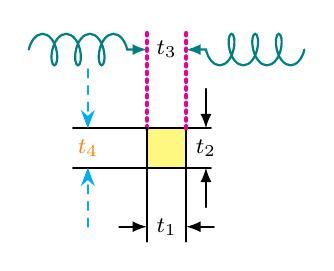
\begin{tikzpicture}
\tkzDefPoints{0/0/A,.5/0/B,.5/.5/C,0/.5/D}
\tkzDrawPolygon[thick,black,fill=yellow!50](A,B,C,D)
\tkzDrawSegment[thick,invertdim={$t_1$,-.75cm,inner xsep=3pt,.35cm}](A,B)

\tkzDrawSegment[thick,invertdim={$t_2$,-.25cm,inner ysep=3pt,.5cm}](B,C)

\tkzDrawSegment[thick,invertdim style/.append style={decorate,decoration={coil,segment length=3mm,amplitude=2mm},teal},invertdim fence style/.append style={magenta,dotted,ultra thick},invertdim={$t_3$,-1cm,inner ysep=3pt,1.5cm}](C,D)

\tkzDrawSegment[thick,invertdim style/.append style={dashed,cyan,-Stealth},invertdim={$t_4$,-.75cm,{inner xsep=3pt,text=orange},.75cm}](D,A)
\end{tikzpicture}
\end{document}
